\documentclass[12pt]{article}

%Technometrics specified margins:

% NOTE: To produce blinded version, replace "0" with "1" below.
\newcommand{\blind}{0}

% DON'T change margins - should be 1 inch all around.
\addtolength{\oddsidemargin}{-.5in}%
\addtolength{\evensidemargin}{-.5in}%
\addtolength{\textwidth}{1in}%
\addtolength{\textheight}{1.3in}%
\addtolength{\topmargin}{-.8in}%
\usepackage{psfrag,epsf,enumerate}

%\usepackage[margin=1.1in]{geometry}
\usepackage{color, amssymb, amsmath,bm,verbatim}
\usepackage{rotating, subfig, setspace, tikz}
\usepackage{graphicx, graphics, epsfig}
\usepackage{multirow,multicol}
\usepackage{natbib}
\newcommand{\tr}{{\mathbf{tr}}}
\newcommand{\rmk}{{\mathcal{K}}}
\newcommand{\I}{{\mathrm{I}}}
\newcommand{\E}{{\mathrm{E}}}
\newcommand{\B}{{\mathcal{B}}}
\newcommand{\bmo}{{\bm{o}}}
\newcommand{\R}{{\mathbb{R}}}
\newcommand{\cov}{{\mathrm{Cov}}}
\newcommand{\Log}{\text{Log}}
\newcommand{\M}{\mathcal{M}}
\newcommand{\refeq}[1]{{eq.~(\ref{#1})}}

\newcommand{\ProjMean}{{\widehat{\bm S}_E}}
\newcommand{\ProjMedian}{{\widetilde{\bm S}_E}}
\newcommand{\GeomMean}{{\widehat{\bm S}_R}}
\newcommand{\GeomMedian}{{\widetilde{\bm S}_R}}
\newcommand{\Rdist}{{d_R}}
\newcommand{\Edist}{{d_E}}

\DeclareMathOperator*{\argmax}{arg\,max}
\DeclareMathOperator*{\argmin}{arg\,min}
\newcommand{\blue}[1]{{\color{blue} #1}}
\newcommand{\red}[1]{{\color{red} #1}}
\newcommand{\green}[1]{{\color{green} #1}}
\newcommand{\hh}[1]{{\color{orange} #1}}

%\pagestyle{plain}
%\bibliographystyle{plainnat}
\bibliographystyle{abbrvnat}
\setcounter{section}{0}
\bibpunct{(}{)}{;}{a}{,}{;}
\graphicspath{{images/}}
%\setlength{\parindent}{0pt}
\begin{document}
\def\spacingset#1{\renewcommand{\baselinestretch}%
{#1}\small\normalsize} \spacingset{1}
%\setcounter{table}{4}
%\setcounter{figure}{9}
\appendix
\spacingset{1.45} % DON'T change the spacing!
\begin{center}
\Large \textbf{Online Supplementary Material for Point Estimation of the Central Orientation of Random Rotations}
\large{Bryan Stanfill, Ulrike Genschel and Heike Hofmann}
\end{center}
\section{Riemannian versus Euclidean Distance in $SO(3)$}
\label{sec:appendix2}
\textit{Result.} For rotation matrices $\bm R_i\in SO(3)$ for $i=1,2,\ldots$ and distances $d_E$ and $d_R$ as defined in the main manuscript in equations (3) and (4), respectively,  it holds that 
\begin{equation}
\label{EvR}
\Edist(\bm R_1,\bm R_2)=2^{3/2}\sin\left(\frac{\Rdist(\bm{R}_1,\bm{R}_2)}{2}\right)
.
\end{equation}
%\begin{figure}[h!]
%\begin{center}
%\begin{tikzpicture}[scale=.9]
%%\draw (0,0) circle (4cm);
%\draw (0,0) node {$\bullet$};
%\draw (3.464102,2) node[anchor =  west]{$\bm R_1\bm v$};
%\draw [->] (0,0)--(4,0);
%%\draw [->] (4,0) arc (0:30:4cm);
%\draw (2,0) node[anchor = north]{$\bm v=(0,1)^\top$};
%\draw (-2,3.46) node[anchor = south east]{$\bm R_2\bm v$};
%\draw [line width=.75mm] (3.464102,2) arc (30:120:4cm);
%\draw[line width=.75mm, color=gray] (-2,3.46)--(3.464102,2);
%\draw [->](0,0) -- (-2,3.464102);
%\draw [->](0,0)--(3.464102,2);
%\draw (1,3.66) node[anchor= south west]{$\Rdist (\bm R_1,\bm R_2)$};
%\draw (-1,1.75) node[anchor= south west]{$\Edist (\bm R_1,\bm R_2)$};
%\draw (0,0) circle (4cm);
%\draw (0,0) node {$\bullet$};
%\draw (0,0)--(4,0) node[anchor =  west]{$o_1$};
%\draw (4,0) node[anchor =  west]{$\bm R_1$};
%\draw (0,0)--(-2,3.46) node[anchor = south east]{$o_2$};
%\draw (-2,3.46) node[anchor = south east]{$\bm R_2$};
%\draw[line width=.75mm] (4,0) arc (0:120:4cm);
%\draw[line width=.75mm, color=gray] (-2,3.46)--(4,0);
%\draw (0,0)--(2,3.46) node[anchor= south west]{$\alpha$};
%\draw (2,3.46) node[anchor= south west]{$\Rdist (\bm R_1,\bm R_2)$};
%\draw (-1.25,0.73) node[anchor= south west]{$\Edist (\bm R_1,\bm R_2)$};
%\draw (3/8,.7)[->] arc (60:120:.75cm);
%\draw (0,1.2) node {$\frac{\alpha}{2}$};
%\draw (0,2.8) node {$\frac{\beta}{2}$};
%\draw (2,0) node[anchor=north]{1};
%\end{tikzpicture}
%\end{center}
%\vspace{-.25cm}
%\caption{An illustration of the Euclidean and Riemannian distance metric on $SO(2)$. To simplify the visualization we use $SO(2)$ in place of $SO(3)$.   $\bm R_1$, $\bm R_2$ are $2\times2$ rotation matrices in $SO(2)$, where $\bm R_1\bm v$ and $\bm R_2\bm v$ are points on the $\mathbb R^2$ unit circle after rotating $\bm v = (0,1)^{\top}$ by  $\bm R_1$ and $\bm R_2$, respectively.  $\Rdist (\bm R_1,\bm R_2)$ is displayed by the curved line (black), $\Edist (\bm R_1,\bm R_2)$ by the straight line (gray).}
%\label{fig:dEvsdG2} 
%\end{figure}

%\noindent In Figure \ref{fig:dEvsdG2} the Riemannian distance between $\bm R_1$ and $\bm R_2\in SO(2)$ is given by $\Rdist(\bm R_1,\bm R_2)$ and is indicated with the thick black arc.  The Euclidean distance is given by $\Edist(\bm R_1,\bm R_2)$ and is indicated by the straight gray line.  Using geometry it is clear that half of the Euclidean distance is the sine of half of the Riemannian distance, i.e.
%\[
%\Edist(\bm R_1,\bm R_2)=2\sin\left(\frac{\Rdist(\bm R_1,\bm R_2)}{2}\right).
%\]

%\noindent We claim that this can be extended to $\bm R_1,\bm R_2 \in SO(3)$ as 
%\begin{equation}\label{EvR}
%\Edist (\bm{R}_1,\bm{R}_2)=2^{3/2}\sin\left(\frac{\Rdist(\bm{R}_1,\bm{R}_2)}{2}\right)
%\end{equation}

\noindent \textit{Proof:} For two rotations $\bm{R}_1,\bm{R}_2\in SO(3)$ recall that if $\tr(\bm R_1^\top\bm R_2)=1+2\cos(r)$ then $|r|=\Rdist(\bm R_1,\bm R_2)$.  When $|r|=0$, the statement in \eqref{EvR} follows directly.  Consider the case $|r|>0$.  By definition we know
\begin{align*}
\Edist (\bm R_1,\bm R_2)^2
&=||\bm R_1-\bm R_2||_F^2\\
&=\tr\left[(\bm R_1-\bm R_2)^\top(\bm R_1-\bm R_2)\right]\\
%&=\tr\left[(\bm R_1^\top-\bm R_2^\top)(\bm R_1-\bm R_2)\right]\\
&=\tr\left[\bm R_1^\top\bm R_1+\bm R_2^\top\bm R_2-\bm R_2^\top\bm R_1-\bm R_1^\top\bm R_2\right]\\
&=\tr\left[2\bm{I}-\bm R_2^\top\bm R_1-\bm R_1^\top\bm R_2\right]\\
&=2\tr(\bm{I})-\tr(\bm R_2^\top\bm R_1)-\tr(\bm R_1^\top\bm R_2)\\
&=6-2\tr(\bm R_1^\top\bm R_2)\\
%&=6-2(1+2\cos(r))\\
&=4-4\cos(|r|)\\
&=8\left(\frac{1-\cos(|r|)}{2}\right)\\
&=8\sin^2\left(\frac{|r|}{2}\right)\\
&=\left[2^{3/2}\sin\left(\frac{|r|}{2}\right)\right]^2\\
&=\left[2^{3/2}\sin\left(\frac{\Rdist(\bm R_1,\bm R_2)}{2}\right)\right]^2.
\end{align*}
Taking square root on both sides gives \eqref{EvR}.

\section{Sampling Processes}
In the following subsection we will briefly illustrate how a sample of random rotations from each of the three rotational distributions (circular-von Mises-based, Cayley and matrix-Fisher) is obtained for the purpose of the simulation study.
\label{sec:appendix1}
\subsection{Circular-von Mises-based distribution}

To simulate a random sample of rotation angles from the circular-von Mises-based distribution we follow the  algorithm proposed by Best and Fisher (1979).  The algorithm is available in the IMSL Library (1991) and is implemented as follows.  Let $\mu=0$ denote the mean of the target angular distribution and $\kappa$ its concentration parameter.  We define constants $a, b$ and $d$ as
$a\equiv 1+\sqrt{1+4\kappa^2},\quad b\equiv(a-\sqrt{2a}),\quad d\equiv(1+b^2)/2b.$
In steps one, two and four we generate three new observations $u_1$, $u_2$ and $u_3$,  each from a uniform distribution defined over the interval $(0,1)$. 
\begin{enumerate}
\item Set $z=\cos(\pi u_1)$, $f=(1+dz)/(z+d)$ and $c=\kappa(d-f)$.
\item If $c(2-c)-u_2>0$ go to step 4.
\item If $\log(c/u_2)+1-c<0$ return to step 1.
\item Set $r=\text{sign}(u_3-0.5)\cos^{-1}(f).$
\end{enumerate}
It follows that  $r$ is distributed according to the circular-von Mises$(\kappa)$ distribution.

\subsection{Cayley distribution}%\hfill

To simulate rotation angles from a Cayley distribution we make use of a result given in Le{\'o}n et al., (2006). If the angle $r$ follows a Cayley distribution it holds that $\frac{1+\cos r}{2} \sim \text{Beta}(\kappa+1/2, 3/2)$.  Hence, angles following the Cayley distribution can be simulated through composition: 
\begin{enumerate}
\item Generate $Z\sim$Bernoulli(0.5) and set  $Y=1-2Z.$
\item Independently generate $X\sim$ Beta$(\kappa+1/2, 3/2).$
\item Set $r= \frac{Y}{2}\cos^{-1}(2X-1).$
\end{enumerate}
Angles $r$ simulated in this fashion follow a Cayley$(\kappa)$ distribution.

\subsection{matrix Fisher distribution}%\hfill

Simulation from the matrix Fisher distribution is achieved through a rejection algorithm.  Let  $\mathrm{C_F}(r|\kappa)$ denote the matrix Fisher density.% as given in Table~\ref{tab:ang.dens}. %and $Y\sim$ Uniform$(-\pi,\pi]$.

\begin{enumerate}
\item Define $M=\frac{1}{2\kappa}e^{2\kappa - 1}\frac{1}{\mathbf{I}_0(2\kappa)-\mathbf{I}_1(2\kappa)}.$
\item Generate $U\sim$ Uniform$(0,1)$ and $Y\sim$ Uniform$(-\pi,\pi]$, where $U$ and $Y$ are independent.
\item If $U<\frac{1}{M}\mathrm{C_F}(Y|\kappa)$, accept $Y$; otherwise return to step (2).
\end{enumerate}

%\subsection{Rotation Matrix Formulation}
%
%Given a set of randomly generated angles of rotation $r_1,\ldots, r_n$, the rotation matrix formulation following from:
%\begin{enumerate}
%\item Generate a point uniformly on the unit sphere
%$$\bm{U}=(u_1,u_2,u_3)^\top=(\sin\theta\cos\phi,\sin\theta\sin\phi,\cos\theta)^\top$$
%where  $0\leq \theta\leq \pi$ and $0\leq \phi\leq 2\pi$.
%\item Given an angle of rotation,$r_i$ , generated as described above from an angular distribution symmetric about 0 and with concentration $\kappa$ rotate $\bm{I}$ about $\bm{U}$ by $r_i$ radians.
%\end{enumerate}


\section{Additional Simulation Study Results}
\label{sec:appendix3}
We expand on some of the results given in Section~5 of the main manuscript by providing additional numerical results to support graphical displays as well as to further clarify the relationship between the different estimators.

\noindent Figure~4 of the main manuscript showed boxplots of the estimation errors for a each of a 1,000 samples of size $n=100$ for all three distributions and choices of the circular variance $\nu$.  We accompany this figure with Table~\ref{tab:alldN100}, which provides numerical summaries of the errors displayed in each boxplot showing the mean estimation error $\overline{\Rdist}(\bm{S}, \widehat{\bm{S}})$ in the $1,000$ simulation runs, the estimated standard error $SE(\overline{\Rdist})$ and the estimated $RMSE$ for each estimator.  Although the boxplots of the estimation errors look very similar in Figure~4, the estimated standard errors in Table \ref{tab:alldN100} suggest that on average some of the estimators differ significantly.  


\begin{table}[h!]
\caption{Mean estimation error, respective standard error and RMSE for $n=100$ based on 1,000 simulation runs. Despite skewness in some of the plotted error distributions the \textit{median estimation error} was quantitatively similar to the mean estimation error and therefore is not reported.
}  
\label{tab:alldN100}
\centering
\scalebox{.85}{
\begin{tabular}{ccccccccccc}
\hline
		&&\multicolumn{3}{c}{\textbf{Cayley}} & \multicolumn{3}{c}{\textbf{matrix Fisher}}  & \multicolumn{3}{c}{\textbf{circular-von Mises}}\\[.15cm] 
  $\nu$ & Estimator && $\overline{\Rdist}(\bm{S}, \widehat{\bm{S}})$  $SE(\overline{\Rdist})$ & RMSE && $\overline{\Rdist}(\bm{S}, \widehat{\bm{S}})$ $SE(\overline{\Rdist}$) & RMSE && $\overline{\Rdist}(\bm{S}, \widehat{\bm{S}})$ $SE(\overline{\Rdist})$ & RMSE \\ \hline
  \hline
 \multirow{4}{*}{0.25} 
 	& $\GeomMean$ && 0.0690 (0.0009) & 0.0752 && 0.0699 (0.0010) & 0.0761 && 0.0744 (0.0010) & 0.0811 \\ 
  	& $\ProjMean$ && 0.0698 (0.0009) & 0.0759 && 0.0695 (0.0009) & 0.0756 && 0.0617 (0.0008) & 0.0671 \\ 
  	& $\GeomMedian$ && 0.0769 (0.0010) & 0.0834 && 0.0747 (0.0010) & 0.0813 && 0.0269 (0.0005) & 0.0310 \\ 
   	&$\ProjMedian$ && 0.0791 (0.0011) & 0.0858 && 0.0766 (0.0010) & 0.0832 && 0.0256 (0.0005) & 0.0296 \\ \hline
  	 \multirow{4}{*}{0.50} 
	&$\GeomMean$ && 0.1086 (0.0014) & 0.1174 && 0.1121 (0.0015) & 0.1219 && 0.1279 (0.0018) & 0.1406 \\ 
  	& $\ProjMean$ && 0.1129 (0.0015) & 0.1222 && 0.1054 (0.0014) & 0.1143 && 0.0894 (0.0012) & 0.0976 \\ 
  	& $\GeomMedian$ && 0.1210 (0.0016) & 0.1313 && 0.1113 (0.0015) & 0.1211 && 0.0426 (0.0008) & 0.0491 \\ 
  	& $\ProjMedian$ && 0.1295 (0.0017) & 0.1407 && 0.1160 (0.0016) & 0.1262 && 0.0379 (0.0007) & 0.0438 \\\hline
  	 \multirow{4}{*}{0.75} 
	& $\GeomMean$ && 0.1398 (0.0018) & 0.1514 && 0.1703 (0.0045) & 0.2225 && 0.2039 (0.0028) & 0.2221 \\ 
  	& $\ProjMean$ && 0.1567 (0.0020) & 0.1695 && 0.1462 (0.0020) & 0.1588 && 0.1276 (0.0017) & 0.1388 \\ 
  	& $\GeomMedian$ && 0.1597 (0.0021) & 0.1729 && 0.1527 (0.0021) & 0.1660 && 0.0687 (0.0012) & 0.0792 \\ 
  	& $\ProjMedian$ && 0.1847 (0.0024) & 0.2000 && 0.1597 (0.0022) & 0.1736 && 0.0547 (0.0010) & 0.0628 \\ 
   \hline
\end{tabular}}
\end{table}

\noindent To establish significant differences more formally we conducted \textit{matched pair} $t$-\textit{tests} (two-sided) for all six pairwise comparisons of the four estimators within a specific simulation setting.  The results are given in Table~\ref{tab:pvalues}. We tested the null hypothesis that the difference in the resulting estimates, on average, is zero against the alternative hypothesis that the difference, on average, is non-zero.  Because differences in the estimation error seem less obvious for the Cayley and matrix-Fisher distribution we conducted tests for both distributions for samples of size 10 and 100 and circular variances of 0.25 and 0.75. 
We suspect that a \textit{matched pair} $t$-\textit{test} based on all of the $B=1,000$ simulations will likely yield statistically significant differences that are an artifact of the size of $B$ as opposed to meaningful and practical differences we also provide the results for (arbitrary) choices of $B=50$ and $B=100.$ For $B=50$ and $B=100$ we base the test on the estimation results for $B$ randomly selected simulation runs and repeated this process 100 times. The reported \textit{p-value} then corresponds to the average \textit{p-value} of these 100 runs. For $B=1,000$ the reported \textit{p-value} is based on all original 1,000 runs. 
We further adjusted the level of significance within each row of Table~\ref{tab:pvalues} using 
a Bonferroni correction for multiple comparisons and therefore, within a set of all six pairwise comparisons, consider \textit{p-values} less than $0.05\div6=0.0083$.  We chose the Bonferroni adjustment because of its simplicity. \\

\noindent From Table \ref{tab:pvalues} we can conclude that for the Cayley distribution the choice of geometry is important when using median type estimators (column 1), but not as important for mean type estimators (column 2) unless the circular variance and sample size is large.  For a given geometry, the difference between mean and median type estimator depends on the level of variability in the data as is the case in the one dimension case (columns 3 and 4).  As for the matrix-Fisher distribution, the choice of estimator does not appear to be overtly significant for any sample size or circular variance.  This is likely due to the fact that this distribution closely resembles the normal distribution on the range $[-\pi,\pi)$ in which case the mean and median are equivalent.

\begin{table}[h!]
\caption{P-values for matched pair t-tests on the average differences between estimators.  Unless $B$ equals 1,000 the reported p-values correspond to the average of 100 p-values based on random samples of size $B$ from 1,000 simulation runs.}
\label{tab:pvalues}
\begin{center}
\scalebox{.89}{
\begin{tabular}{ccccrrrrrr}
  \hline\\[-4pt]
 Distribution & $\nu$ & $n$ & $B$ &$\ProjMedian-\GeomMedian$ & $\ProjMean-\GeomMean$ & $\ProjMean-\ProjMedian$ & $\GeomMean-\GeomMedian$ & $\ProjMean-\GeomMedian$ & $\ProjMedian-\GeomMean$ \\ 
 \hline\hline
 \multirow{12}{*}{Cayley} & \multirow{6}{*}{0.25} & \multirow{3}{*}{10} & 50 & \textbf{0.0012} & 0.4106 & 0.0181 & 0.0591 & 0.0385 & 0.0298 \\ 
  &  &  & 100 & $<$\textbf{0.0001} & 0.3438 & \textbf{0.0004} & \textbf{0.0040} & \textbf{0.0022} & \textbf{0.0008} \\ 
  &  &  & 1000 & $<$\textbf{0.0001} & \textbf{0.0022} & $<$\textbf{0.0001} & $<$\textbf{0.0001} & $<$\textbf{0.0001} & $<$\textbf{0.0001} \\ \cline{3-10}
  &  & \multirow{3}{*}{100} & 50 & $<$\textbf{0.0001} & 0.2937 & 0.0110 & 0.0360 & 0.0248 & 0.0179 \\ 
  &  &  & 100 & $<$\textbf{0.0001} & 0.1356 & \textbf{0.0002} & \textbf{0.0012} & \textbf{0.0007} & \textbf{0.0003} \\ 
  &  &  & 1000 &$<$\textbf{0.0001} & $<$\textbf{0.0001} & $<$\textbf{0.0001} & $<$\textbf{0.0001} & $<$\textbf{0.0001} & $<$\textbf{0.0001} \\ \cline{2-10}
  &  \multirow{6}{*}{0.75}& \multirow{3}{*}{10} & 50 & \textbf{0.0001} & 0.0343 & \textbf{0.0008} & 0.0376 & 0.3306 & \textbf{0.0005} \\ 
  &  &  & 100 & $<$\textbf{0.0001} & \textbf{0.0015} & $<$\textbf{0.0001} & \textbf{0.0018} & 0.2848 & $<$\textbf{0.0001} \\ 
  &  &  & 1000 & $<$\textbf{0.0001} & $<$\textbf{0.0001} & $<$\textbf{0.0001} & $<$\textbf{0.0001} & $<$\textbf{0.0001} & $<$\textbf{0.0001} \\ \cline{3-10}
  &  & \multirow{3}{*}{100} & 50 & $<$\textbf{0.0001} & \textbf{0.0017} & \textbf{0.0001} & \textbf{0.0024} & 0.3292 &$<$\textbf{0.0001} \\ 
  &  &  & 100 & $<$\textbf{0.0001} & $<$\textbf{0.0001} & $<$\textbf{0.0001} & $<$\textbf{0.0001} & 0.3046 & $<$\textbf{0.0001} \\ 
  &  &  & 1000 & $<$\textbf{0.0001} & $<$\textbf{0.0001} & $<$\textbf{0.0001} & $<$\textbf{0.0001} & $<$\textbf{0.0001} & $<$\textbf{0.0001} \\[5pt] \hline\\[-4pt]
  & \multirow{6}{*}{0.25} & \multirow{3}{*}{10} & 50 & 0.0116 & 0.5032 & 0.0791 & 0.2135 & 0.1338 & 0.1394 \\ 
  &  &  & 100 & \textbf{0.0012} & 0.3815 & 0.0213 & 0.1171 & 0.0540 & 0.0586 \\ 
  &  &  & 1000 & $<$\textbf{0.0001} & \textbf{0.0008} & $<$\textbf{0.0001} & $<$\textbf{0.0001} & $<$\textbf{0.0001} & $<$\textbf{0.0001} \\ \cline{3-10}
  &  & \multirow{3}{*}{100} & 50 & \textbf{0.0072} & 0.4314 & 0.0773 & 0.2313 & 0.1200 & 0.1620 \\ 
  &  &  & 100 & \textbf{0.0001} & 0.4250 & \textbf{0.0047} & 0.0603 & 0.0143 & 0.0244 \\ 
  matrix-&  &  & 1000 & $<$\textbf{0.0001} & 0.0303 & $<$\textbf{0.0001} & $<$\textbf{0.0001} & $<$\textbf{0.0001} & $<$\textbf{0.0001} \\ \cline{2-10}
  Fisher& \multirow{6}{*}{0.75} & \multirow{3}{*}{10} & 50 & 0.1027 & 0.1864 & 0.0842 & 0.3483 & 0.3509 & 0.4652 \\ 
  &  &  & 100 & 0.0205 & 0.0730 &\textbf{0.0075} & 0.2476 & 0.1666 & 0.5001 \\ 
  &  &  & 1000 & $<$\textbf{0.0001} & $<$\textbf{0.0001} & $<$\textbf{0.0001} & $<$\textbf{0.0001} & $<$\textbf{0.0001} & 0.1050 \\ \cline{3-10}
  &  & \multirow{3}{*}{100} & 50 & 0.1475 & 0.0586 & 0.0559 & 0.2005 & 0.2296 & 0.4738 \\ 
  &  &  & 100 & 0.0419 & \textbf{0.0081} & \textbf{0.0056} & 0.0747 & 0.0768 & 0.4437 \\ 
  &  &  & 1000 & $<$\textbf{0.0001} & $<$\textbf{0.0001} & $<$\textbf{0.0001} & $<$\textbf{0.0001} & $<$\textbf{0.0001} & 0.0198 \\ 
   \hline
\end{tabular}}
\end{center}
\end{table}

\noindent Figure \ref{fig:NBoxes} illustrates the behavior of the estimators as a function of the sample size. Results are displayed for  $\nu=0.75$ at each sample size. As to be expected, the estimation error decreases as the sample size increases for all three distributions. For small samples, e.g., $n=10$, the estimator exhibiting the largest amount of variability is the geodesic mean $\GeomMean$. This behavior is consistent for all three distributions.  While the estimator's variability lessens considerably for the Cayley and matrix Fisher distribution as $n$ increases, the estimator remains the most variable estimator for the circular-von Mises-based distribution.  A possible explanation for this behavior is that the algorithm to estimate $\GeomMean$ uses a random sample point in its initiating step.  For small samples or samples with several extreme observations it is likely to start the algorithm far from the true center, which in turn may cause the algorithm to get stuck in a local minimum and to fail to converge globally.  In practice we suggest the algorithm be started at some other location estimate of $\bm S$ such as the $\ProjMean$. In simulations where $\ProjMean$ was used as a starting point for the algorithm we observed  similar results with less variability in the estimates of $\GeomMean$, but for the purpose of a fair comparison in this study we started the algorithm at a random sample point.


\begin{figure}[h!]
\centering
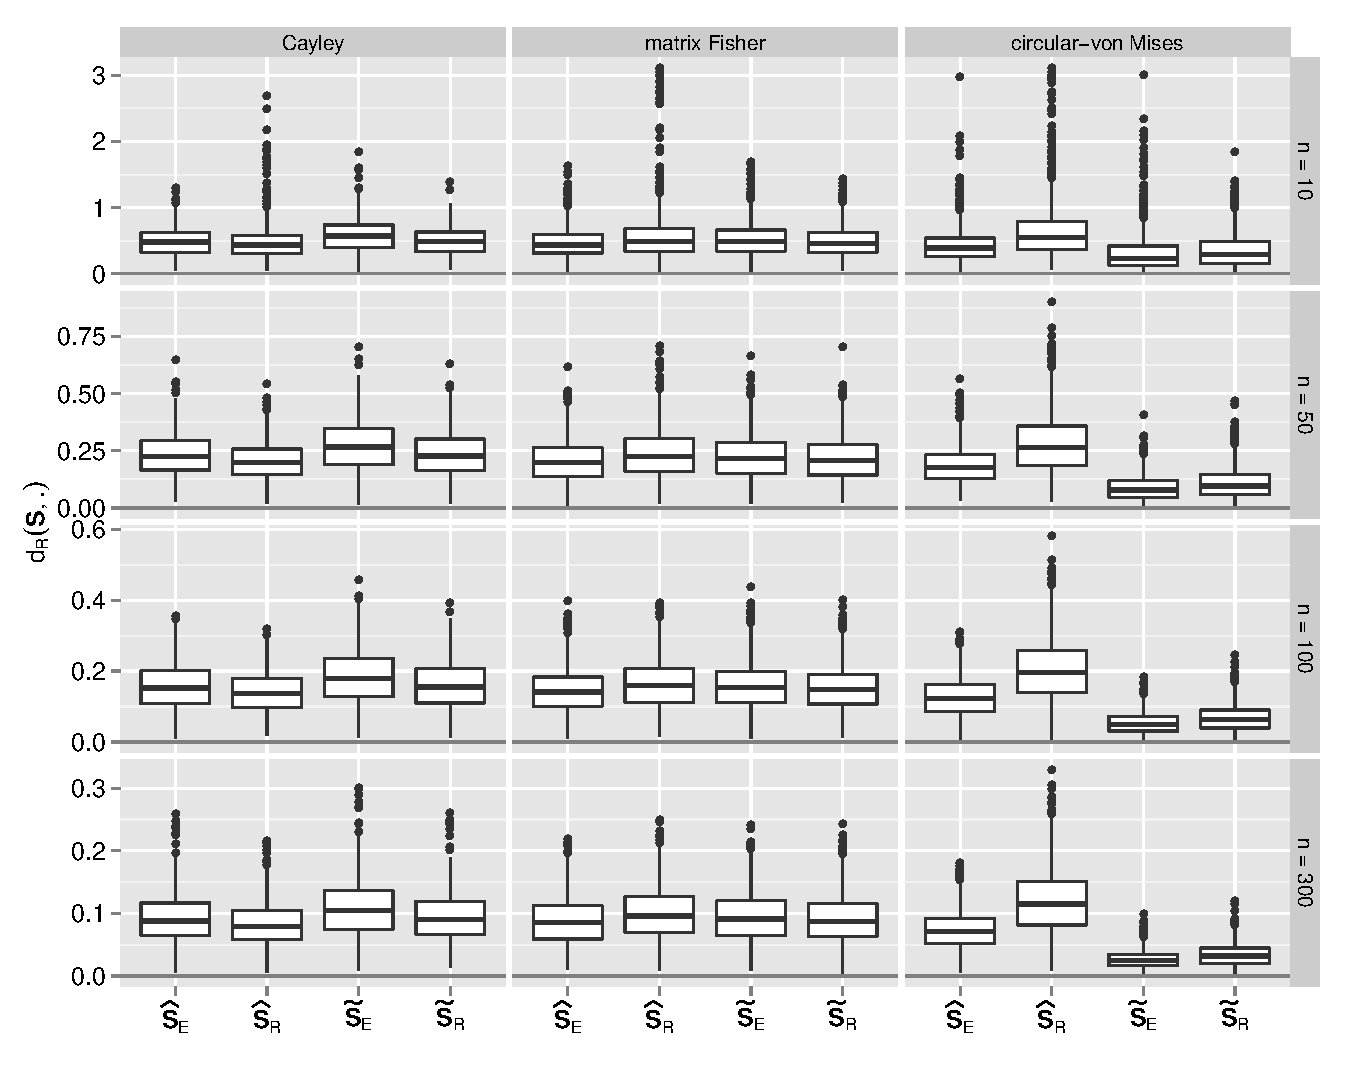
\includegraphics[width=1\textwidth]{Nu75AllNBoxes.pdf}
\caption{Boxplots of the estimation error for each rotation distribution and level of $n$,  $\nu=0.75$.}
\label{fig:NBoxes}
\end{figure}


\noindent In Figure 7 of the main manuscript we examined how the choice of geometry (Riemannian versus Euclidean) affected the estimation error under both types of loss functions $L
_1$ and $L_
2$.  Tables~\ref{tab:percL1} and \ref{tab:percL2} support Figure 7 with an exact count (expressed as a percentage) of how often $\Rdist$ resulted in a smaller estimation error than $\Edist$.  Additionally, we give the average amount by which the $\Rdist-$ and $\Edist-$based estimates deviate from one another (along with a standard error estimate).  We denote the latter quantity by $\bar\delta$ where  $\delta=\Rdist(\ProjMedian,\bm S)-\Rdist(\GeomMedian,\bm S)$.   

\begin{table}[h]
\caption{Average reduction in estimation error by using $\GeomMedian$ instead of $\ProjMedian$, $\delta=\Rdist(\ProjMedian,\bm S) - \Rdist(\GeomMedian,\bm S)$ with standard error and percentage of samples for which $\Rdist(\GeomMedian,\bm S) < \Rdist(\ProjMedian,\bm S)$.}
\label{tab:percL1}
\centering
\scalebox{0.92}{
\begin{tabular}{crccccccccc}
  \hline
  %&&&\multicolumn{3}{c}{} & &\multicolumn{3}{c}{\textbf{matrix} } &&\multicolumn{3}{c}{\textbf{circular-}}\\
    &&&\multicolumn{2}{c}{\textbf{Cayley}} & &\multicolumn{2}{c}{\textbf{matrix Fisher}} & &\multicolumn{2}{c}{\textbf{circular-von Mises}}\\ 
\rule[2mm]{0mm}{3mm} 
  $\nu$&  $n$ && $\bar{\delta}$ (SE) & \% & & $\bar{\delta}$ (SE) & \% & & $\bar{\delta}$ (SE) & \% \\ 
  \hline \hline
\multirow{4}{*}{0.25}  
 &    10 && 0.0078 (0.0004) & 0.7430 && 0.0060 (0.0004) & 0.7250 && -0.0053 (0.0006) & 0.3280 \\ 
 &    50 && 0.0031 (0.0001) & 0.7830 && 0.0024 (0.0001) & 0.6970 && -0.0018 (0.0001) & 0.3270 \\ 
 &   100 && 0.0022 (0.0001) & 0.7890 && 0.0018 (0.0001) & 0.7120 && -0.0013 (0.0001) & 0.3080 \\ 
 &   300 && 0.0012 (0.0001) & 0.7810 && 0.0010 (0.0001) & 0.7110 && -0.0008 (0.0001) & 0.2840 \\
\hline
\multirow{4}{*}{0.50}   
  &    10 && 0.0315 (0.0016) & 0.7720 && 0.0171 (0.0017) & 0.6620 && -0.0192 (0.0020) & 0.3350 \\ 
  &    50 && 0.0126 (0.0005) & 0.8110 && 0.0055 (0.0006) & 0.6200 && -0.0081 (0.0005) & 0.2820 \\ 
  &   100 && 0.0085 (0.0003) & 0.8090 && 0.0047 (0.0004) & 0.6600 && -0.0047 (0.0003) & 0.3020 \\ 
  &   300 && 0.0049 (0.0002) & 0.8040 && 0.0024 (0.0002) & 0.6580 && -0.0027 (0.0001) & 0.2550 \\ 
\hline
\multirow{4}{*}{0.75}   
  &    10 && 0.0895 (0.0042) & 0.8210 && 0.0340 (0.0040) & 0.6330 && -0.0396 (0.0062) & 0.3220 \\ 
  &    50 && 0.0366 (0.0011) & 0.8660 && 0.0093 (0.0013) & 0.5970 && -0.0213 (0.0011) & 0.2380 \\ 
  &   100 && 0.0250 (0.0008) & 0.8580 && 0.0069 (0.0009) & 0.6030 && -0.0140 (0.0007) & 0.2400 \\ 
  &   300 && 0.0140 (0.0004) & 0.8500 && 0.0033 (0.0005) & 0.5890 && -0.0072 (0.0003) & 0.2180 \\   \hline
\end{tabular}}
\end{table}

\begin{table}[h!]
\caption{Average reduction in estimation error by using $\GeomMean$ instead of $\ProjMean$, $\delta=\Rdist(\ProjMean,\bm S) - \Rdist(\GeomMean,\bm S)$ with standard error and percentage of samples for which $\Rdist(\GeomMean,\bm S) < \Rdist(\ProjMean,\bm S)$.}  \label{tab:percL2}
\centering
\scalebox{0.92}{
\begin{tabular}{crcccccccccccc}
  \hline
  %& &&\multicolumn{3}{c}{} & &\multicolumn{3}{c}{\textbf{matrix} } &&\multicolumn{3}{c}{\textbf{circular-}}\\
    &&&\multicolumn{2}{c}{\textbf{Cayley}} & &\multicolumn{2}{c}{\textbf{matrix Fisher}} & &\multicolumn{2}{c}{\textbf{circular-von Mises}}\\ 
\rule[2mm]{0mm}{3mm} 
  $\nu$&  $n$ && $\bar{\delta}$ (SE) & \% & & $\bar{\delta}$ (SE) & \% & & $\bar{\delta}$ (SE) & \% \\  
  \hline \hline
\multirow{4}{*}{0.25} 
 &    10 && 0.0011 (0.0004) & 0.5210 && -0.0016 (0.0005) & 0.4500 && -0.0344 (0.0030) & 0.1280 \\ 
 &    50 && 0.0007 (0.0002) & 0.5310 && -0.0011 (0.0003) & 0.4350 && -0.0156 (0.0007) & 0.2090 \\ 
 &   100 && 0.0007 (0.0001) & 0.5650 && -0.0004 (0.0002) & 0.4690 && -0.0126 (0.0005) & 0.2010 \\ 
 &   300 && 0.0005 (0.0001) & 0.5880 && -0.0003 (0.0001) & 0.4860 && -0.0070 (0.0003) & 0.2390 \\\hline
\multirow{4}{*}{0.50}  
 &    10 && 0.0099 (0.0013) & 0.5920 && -0.0178 (0.0027) & 0.4340 && -0.1011 (0.0051) & 0.1570 \\ 
  &    50 && 0.0069 (0.0006) & 0.6450 && -0.0107 (0.0011) & 0.3920 && -0.0545 (0.0018) & 0.1450 \\ 
  &   100 && 0.0043 (0.0004) & 0.6420 && -0.0067 (0.0008) & 0.3930 && -0.0385 (0.0013) & 0.1620 \\ 
  &   300 && 0.0025 (0.0002) & 0.6420 && -0.0040 (0.0004) & 0.3930 && -0.0234 (0.0007) & 0.1570 \\ \hline
\multirow{4}{*}{0.75}  
  &    10 && 0.0163 (0.0062) & 0.6680 && -0.0958 (0.0105) & 0.3570 && -0.2101 (0.0113) & 0.1710 \\ 
  &    50 && 0.0257 (0.0012) & 0.7410 && -0.0356 (0.0045) & 0.3380 && -0.0955 (0.0032) & 0.1500 \\ 
  &   100 && 0.0169 (0.0009) & 0.7350 && -0.0240 (0.0043) & 0.3460 && -0.0763 (0.0021) & 0.1110 \\ 
  &   300 && 0.0091 (0.0005) & 0.7280 && -0.0124 (0.0009) & 0.3440 && -0.0446 (0.0012) & 0.1270 \\
   \hline
\end{tabular}}
\end{table}



%\begin{table}[h!]
%\caption{Results from an analysis of variance on the log transformed error data for $n=100$ and $\nu=0.25$ and treating distributions as blocks.  From this we can conclude that there is a statistically significant difference between the estimators.}
%\begin{center}
%\begin{tabular}{lrrrrr}
%  \hline
% & Df & Sum Sq & Mean Sq & F value & Pr($>$F) \\ 
%  \hline
%Distribution       & 2 & 927.61 & 463.80 & 1371.56 & $<1\times 10^{-5}$ \\ 
%Estimator   & 3 & 228.43 & 76.14 & 225.17 & $<1\times 10^{-5}$ \\ 
%Residuals   & 11994 & 4055.85 & 0.34 &  &  \\ \hline
%Total & 11999 & 5211.88 &&&\\
%   \hline
%\end{tabular}
%\end{center}
%\end{table}


\section{Sphere plots}
\label{sec:appendix.eyeballs}
Figures \ref{fig:eye-cayley} to \ref{fig:eye-vmises} show sphere plots for 100 samples from each of the Cayley, matrix Fisher and circular-von Mises distribution. The concentration parameter $\kappa$ in each distribution is chosen such that the samples have a circular variance of $\nu = 0.25$. The concentration of rotation matrices under circular-von Mises sampling is much higher to the origin (center of the circles) than for the two other distributions.


\begin{figure}
\centering
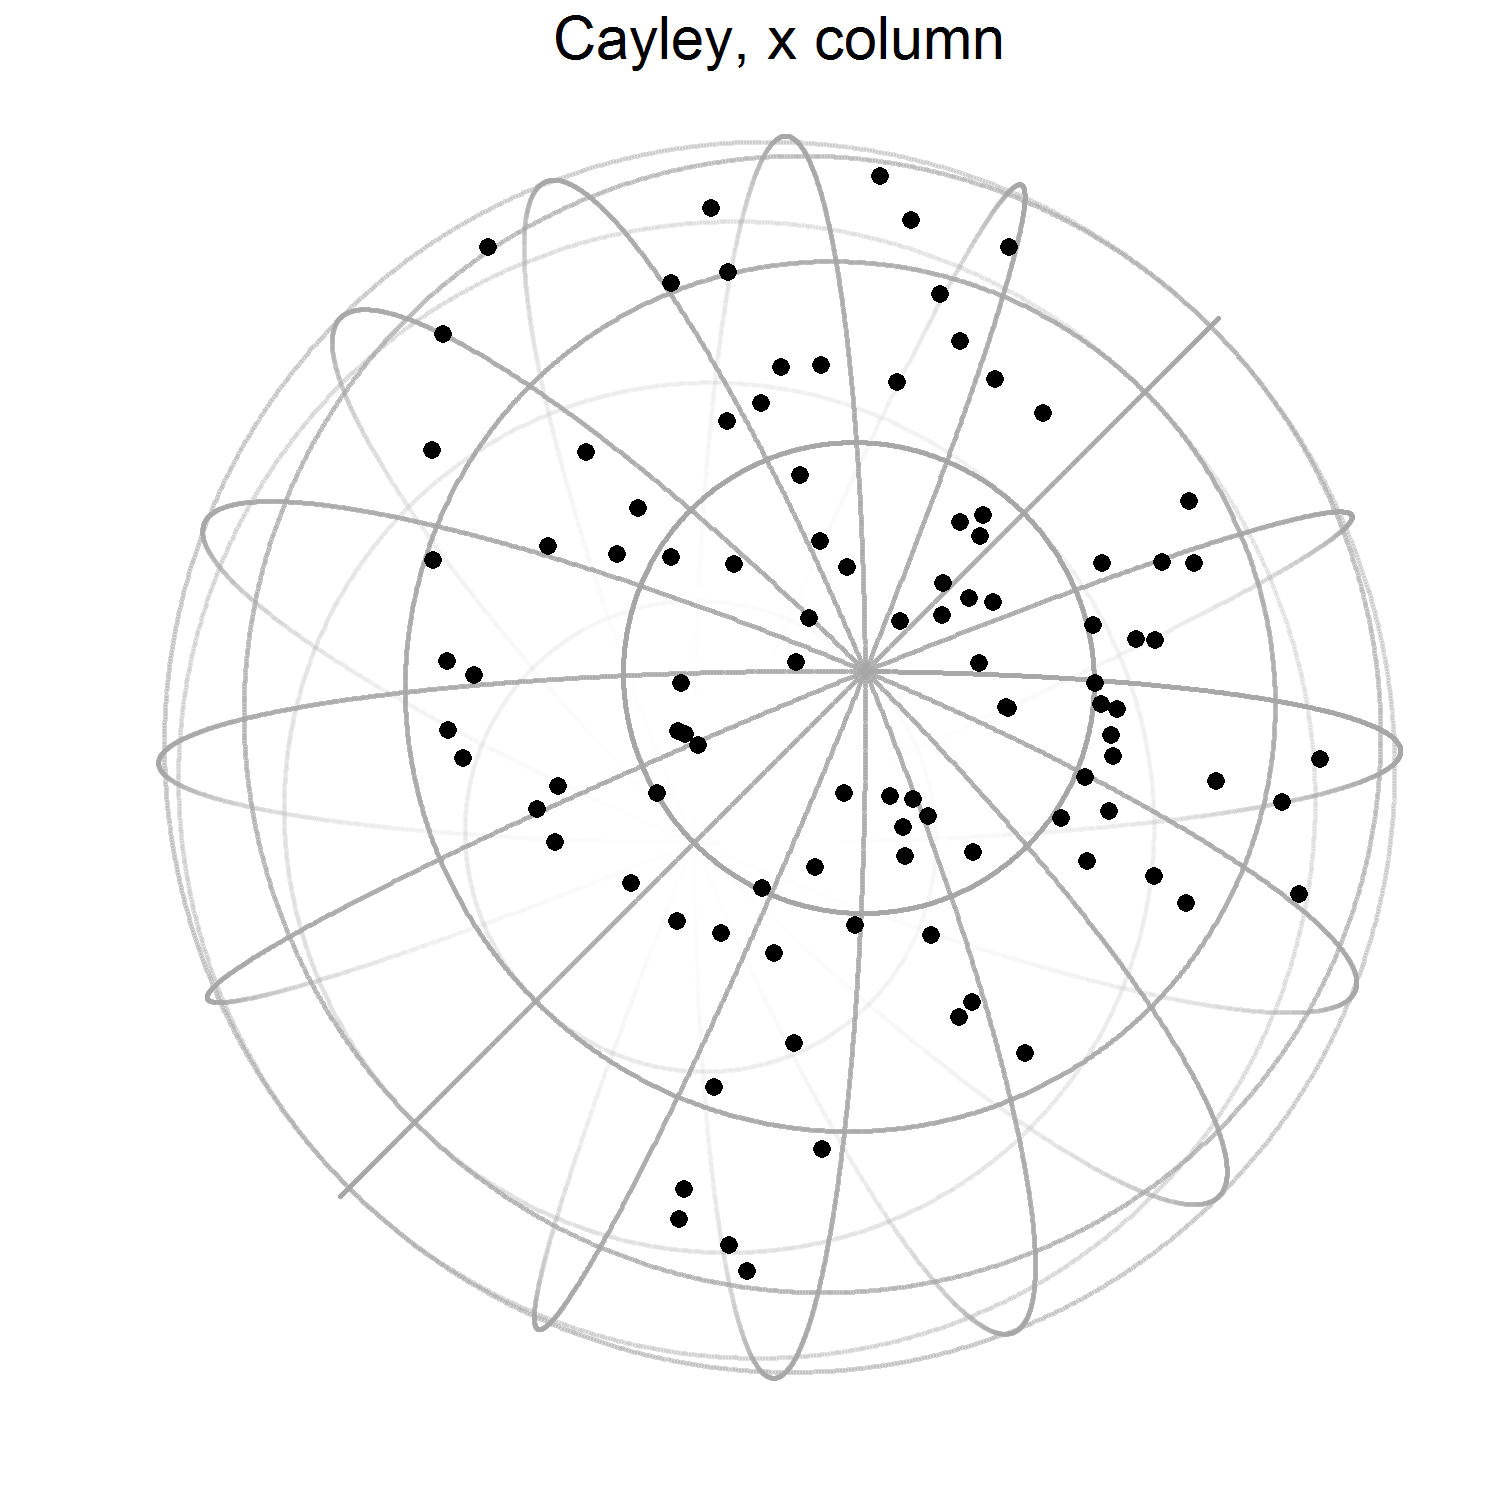
\includegraphics[width=.3\linewidth]{eye-cayley}
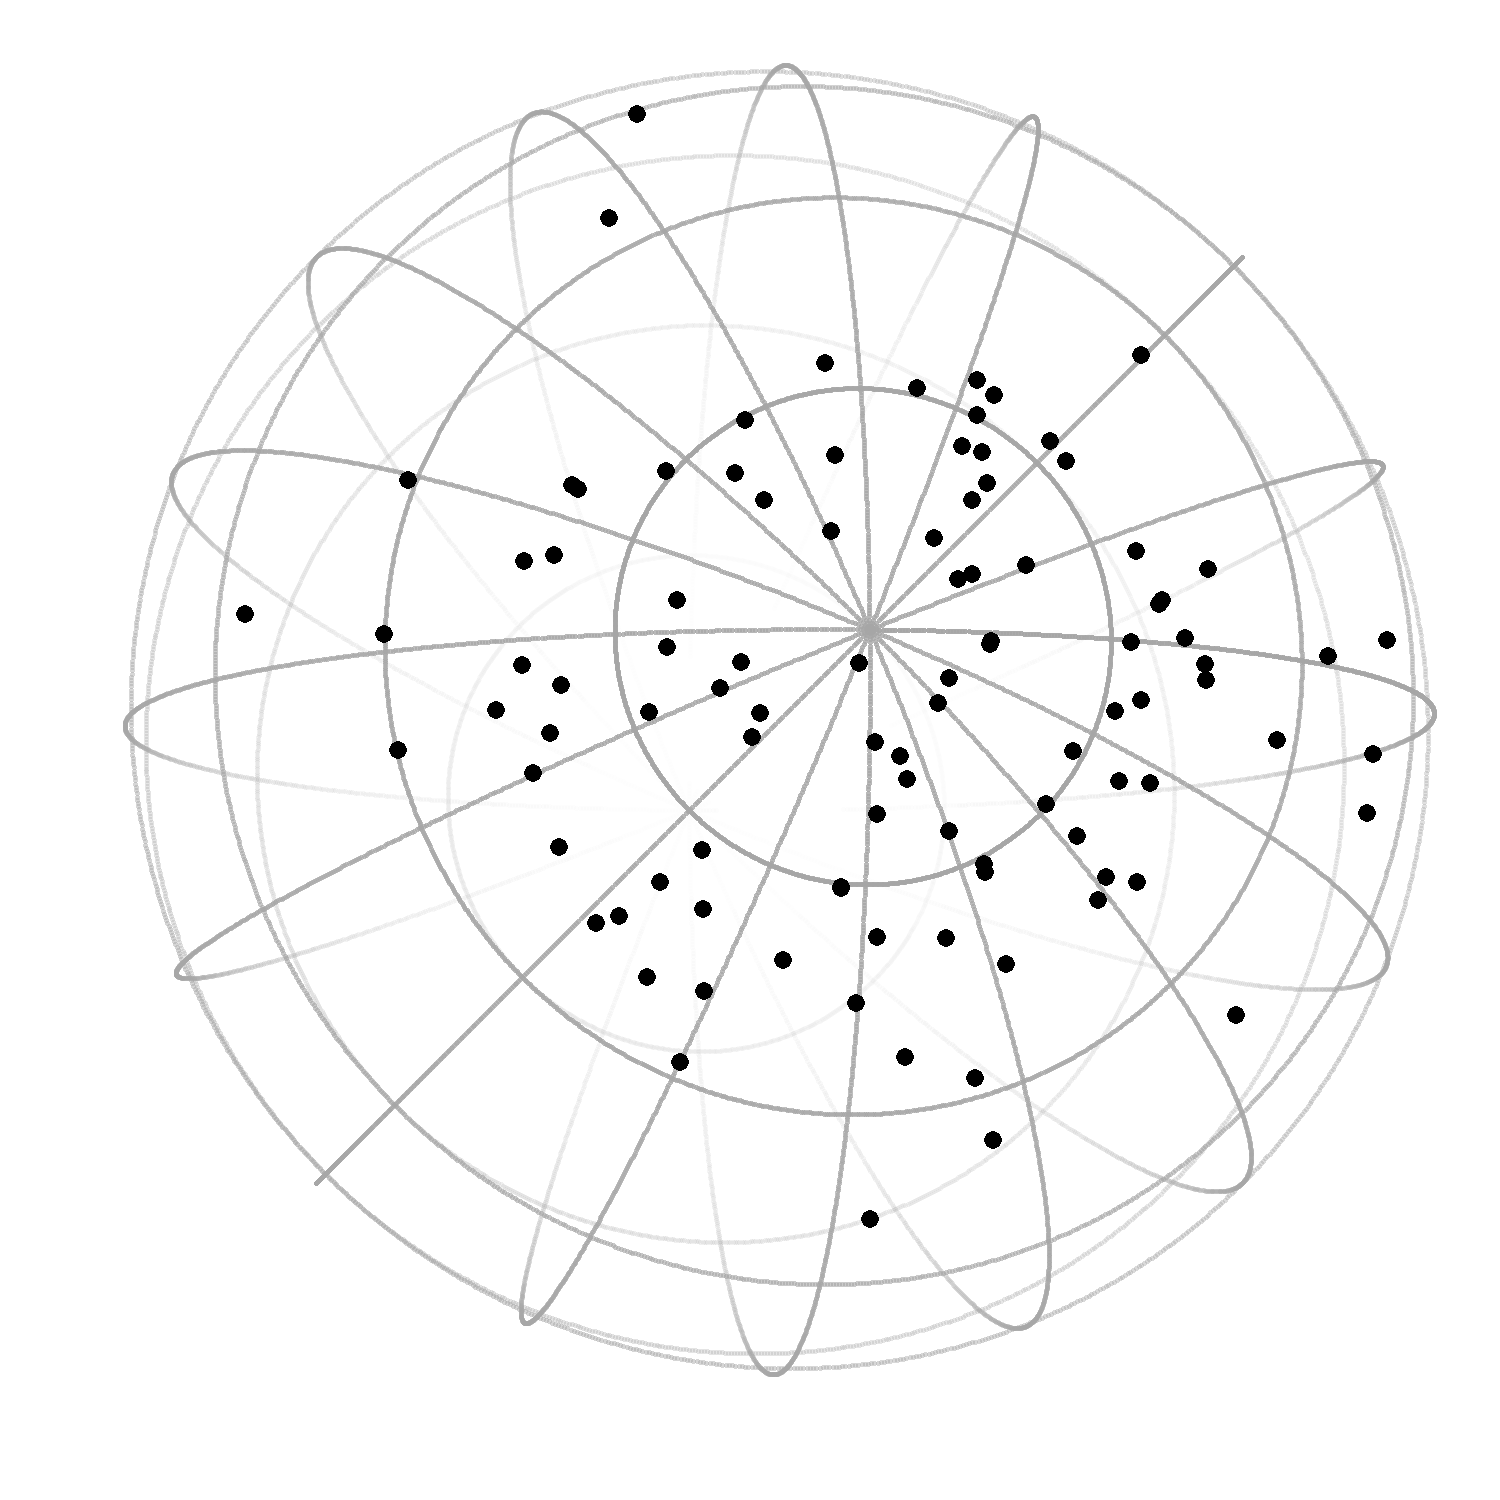
\includegraphics[width=.3\linewidth]{eye-cayley-2}
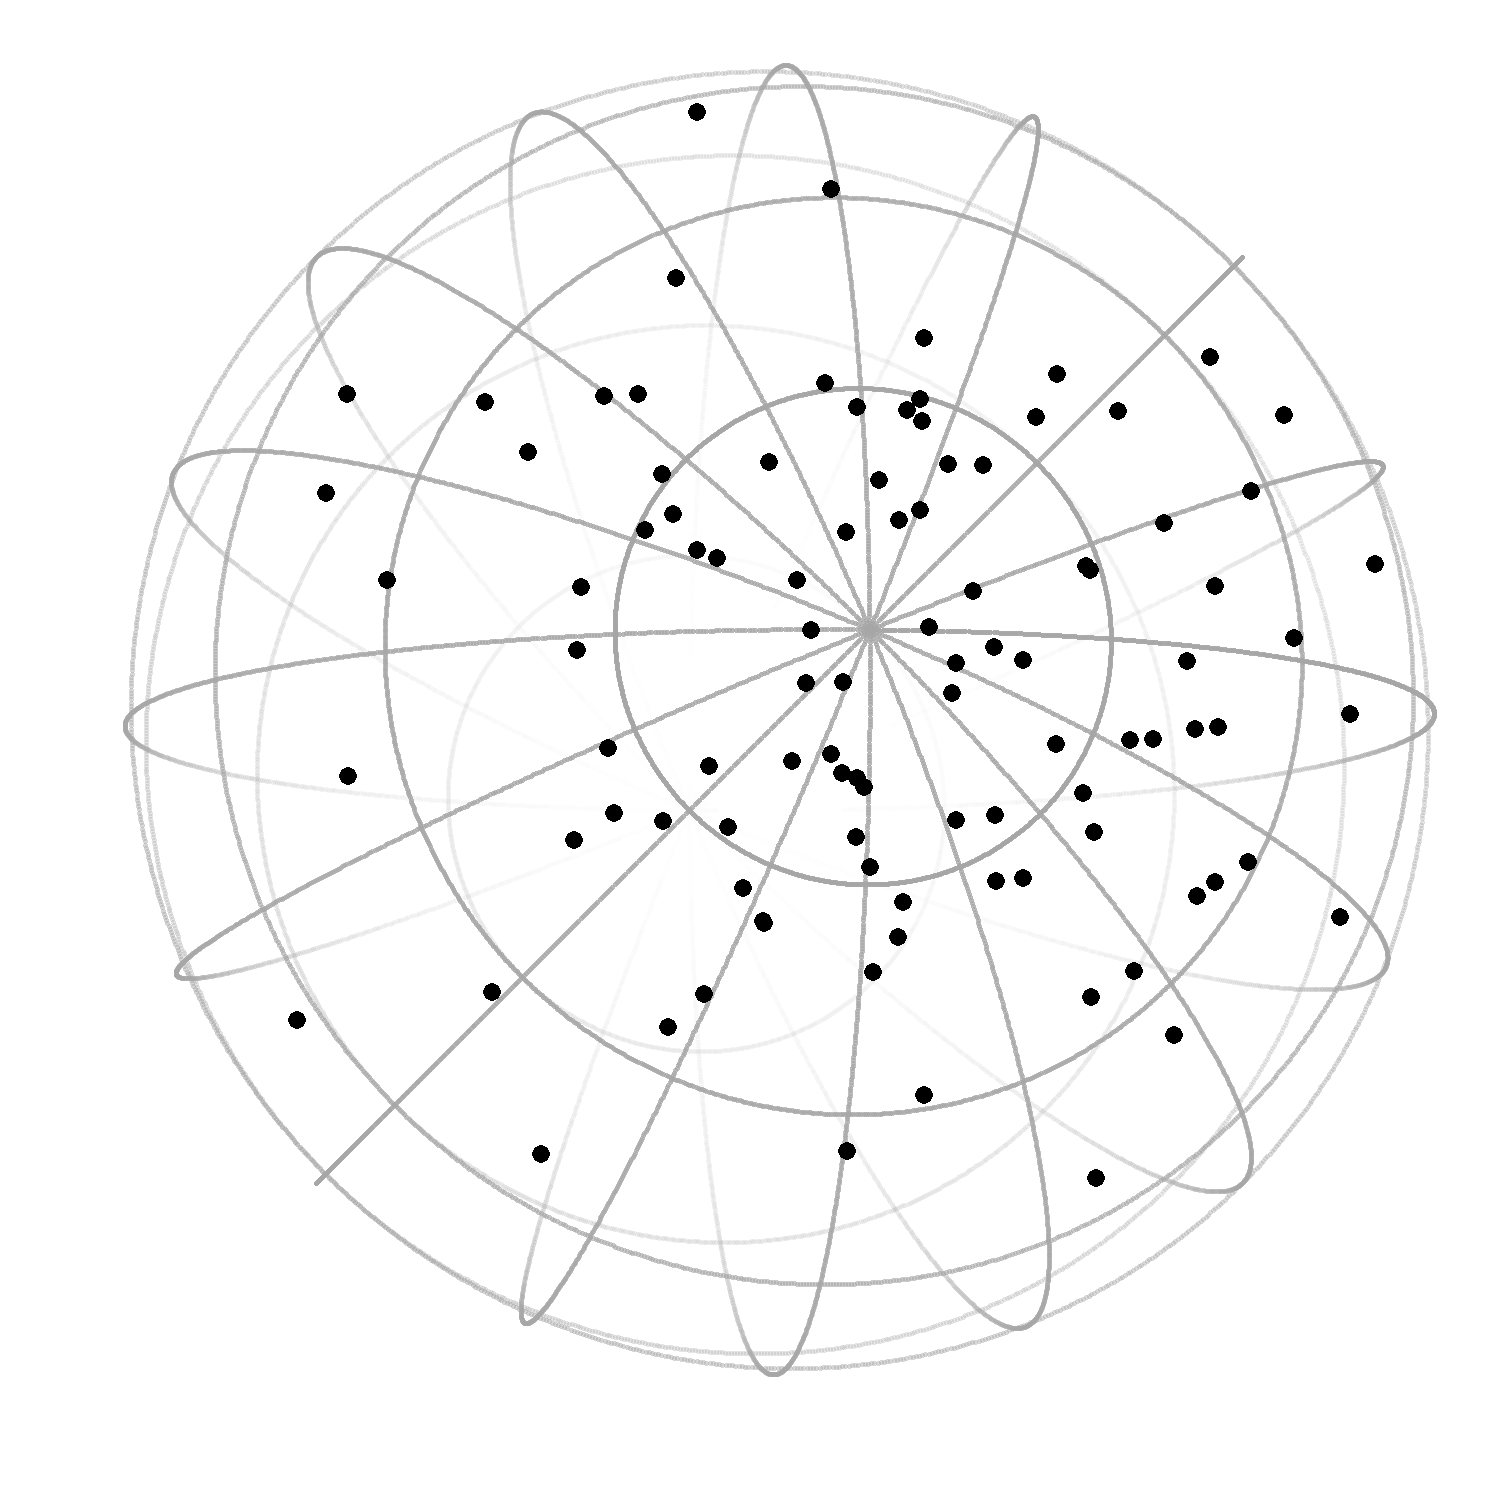
\includegraphics[width=.3\linewidth]{eye-cayley-3}
\caption{\label{fig:eye-cayley}Sphere plots for a sample of 100 rotations from a Cayley distribution with circular variance $\nu=0.25$}
\end{figure}
\begin{figure}
\centering
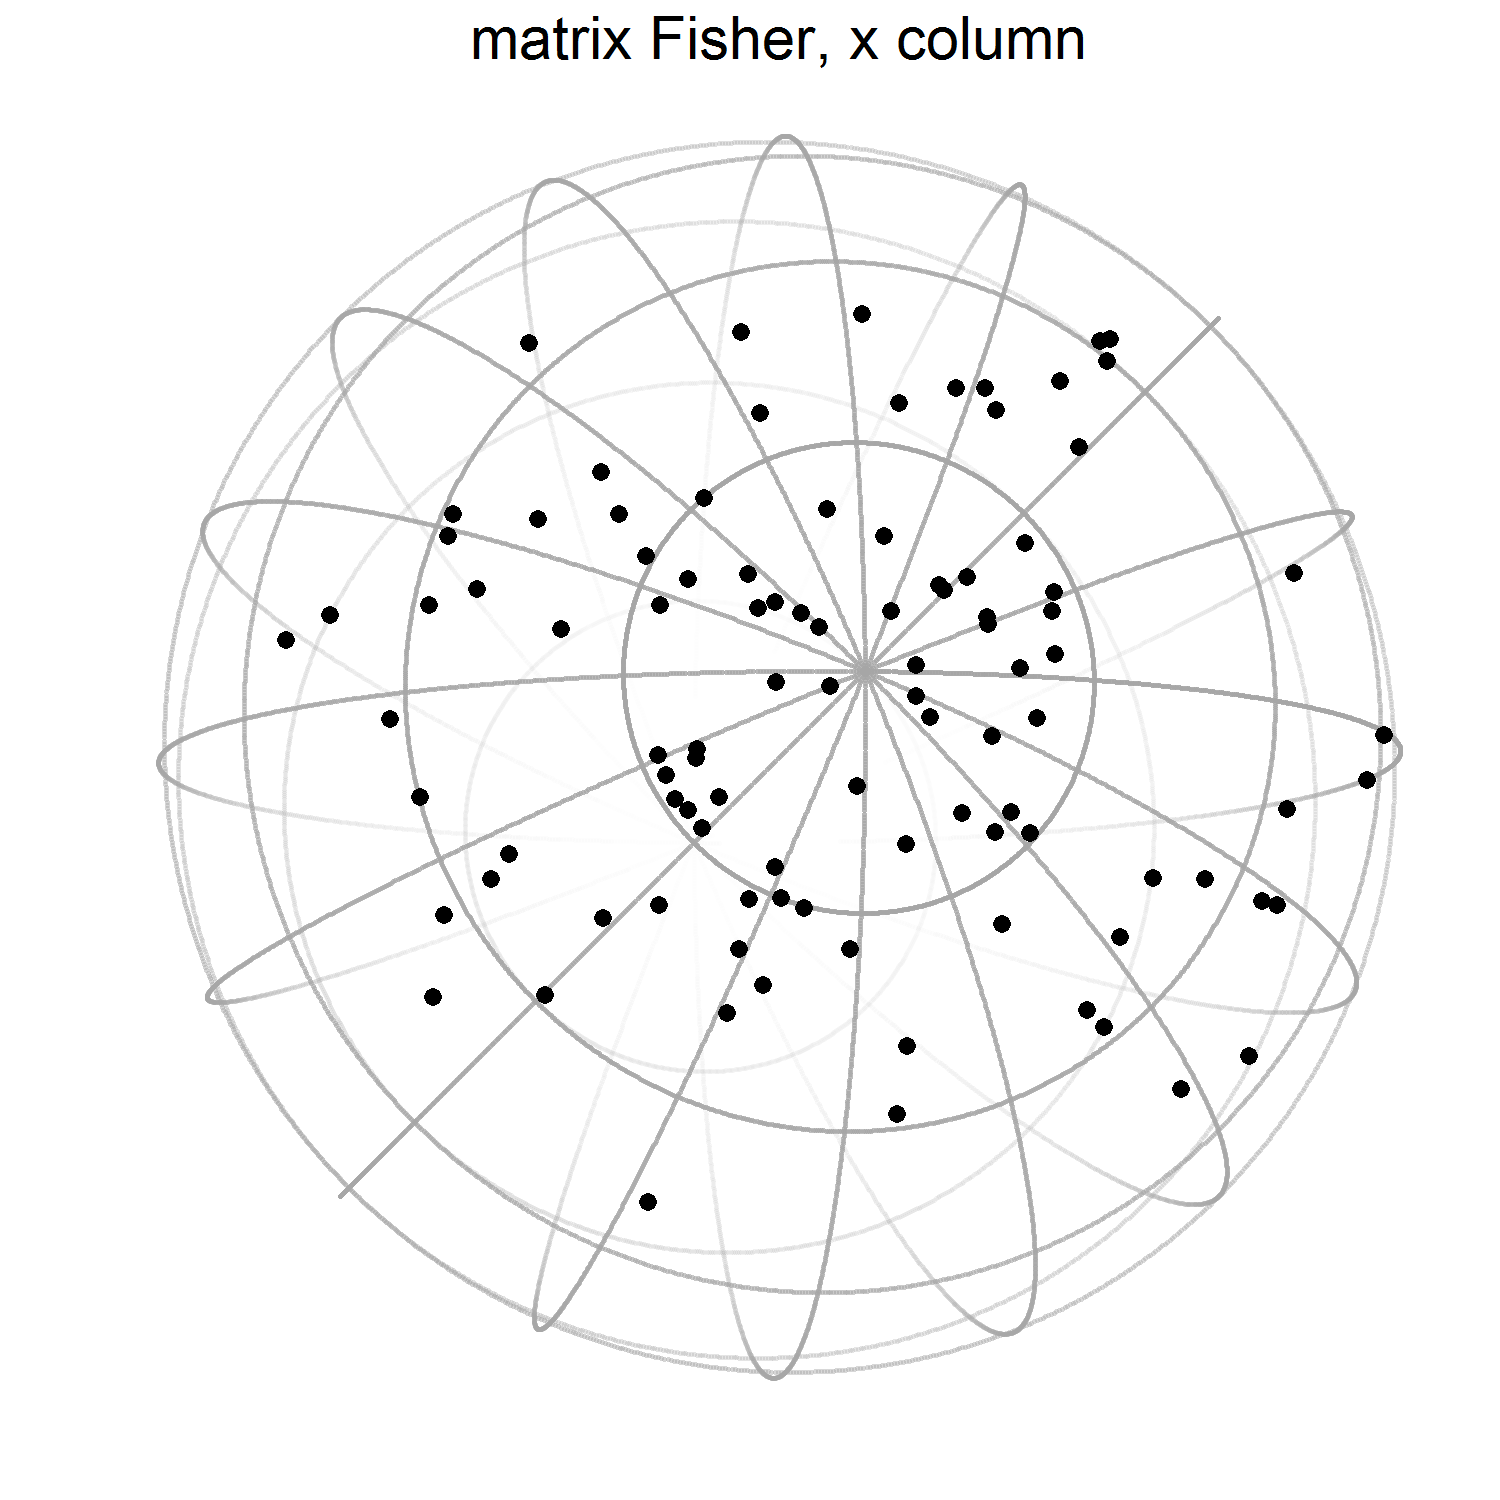
\includegraphics[width=.3\linewidth]{eye-fisher}
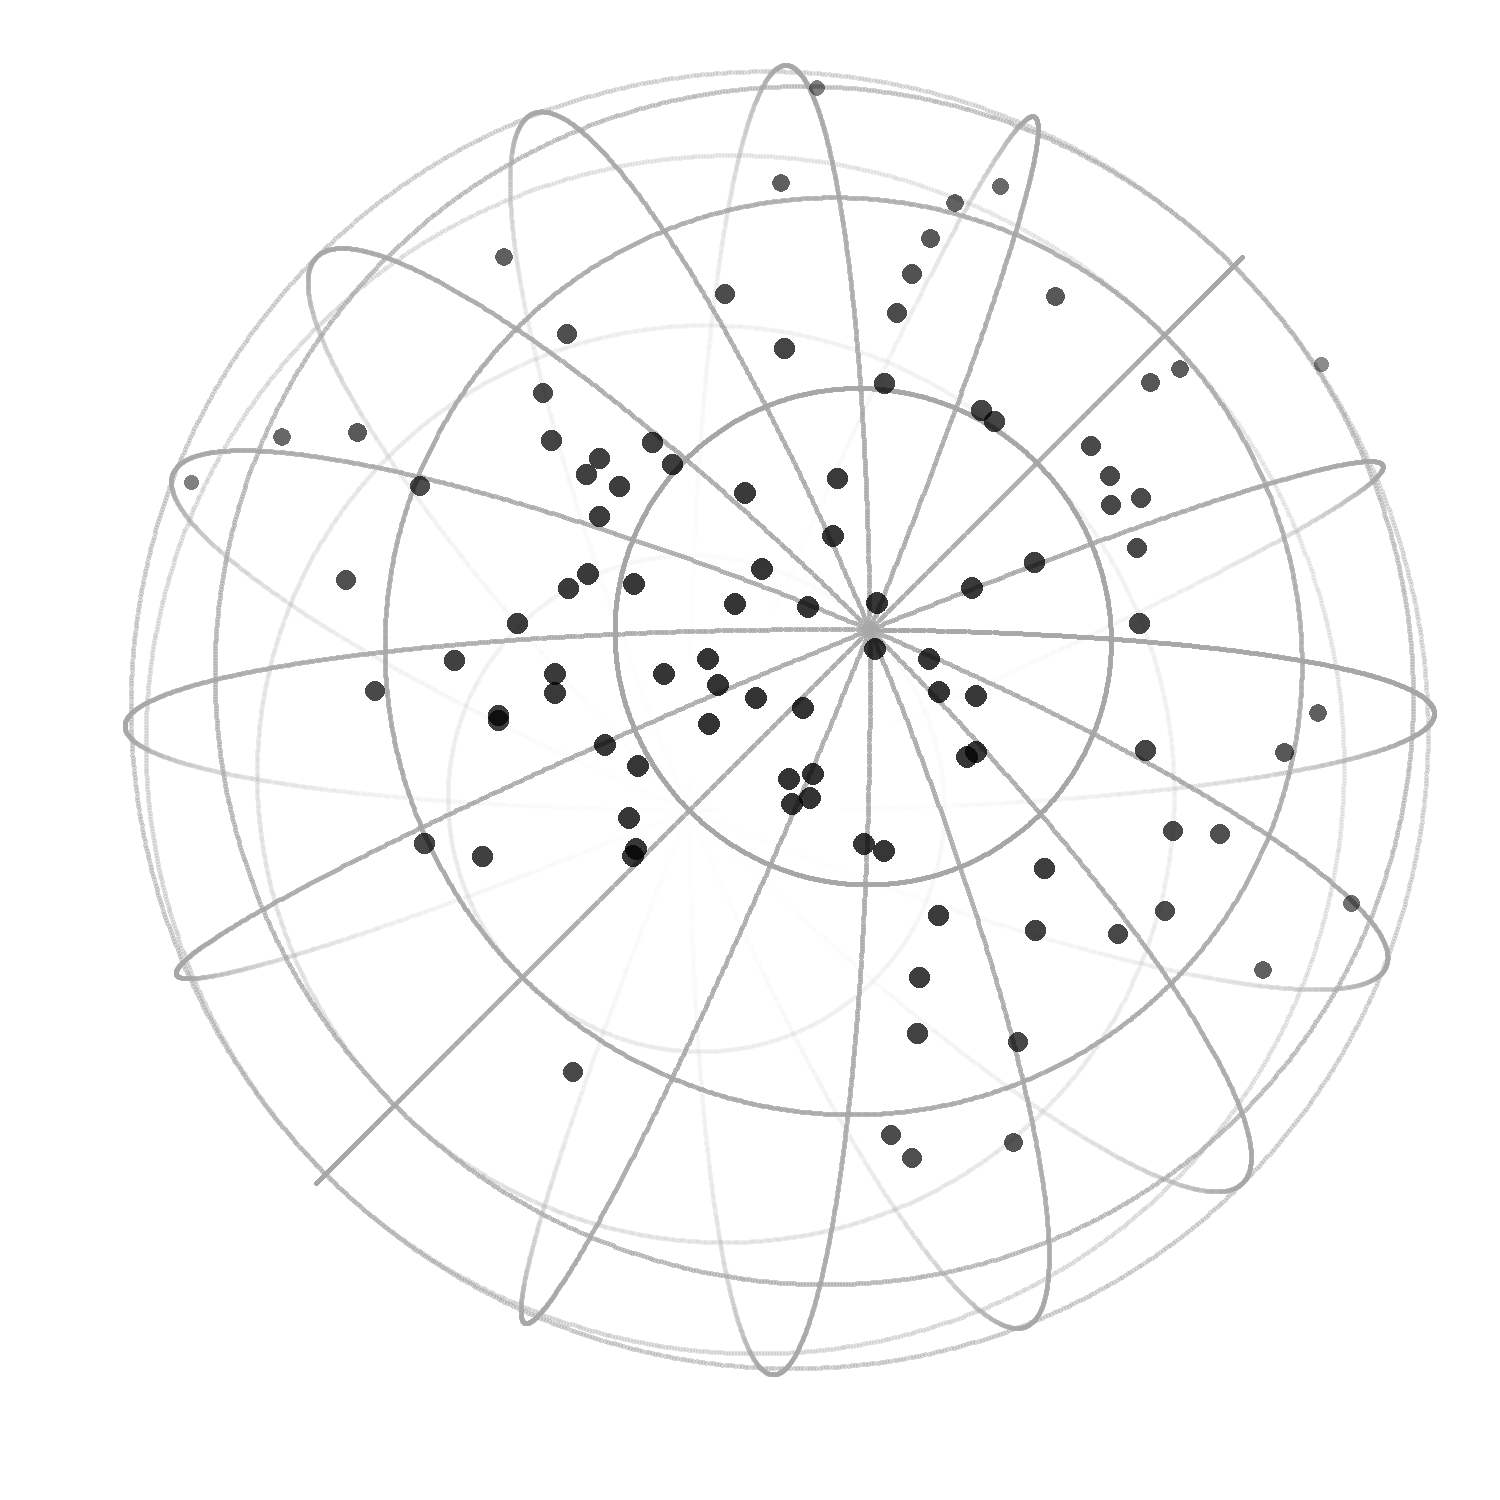
\includegraphics[width=.3\linewidth]{eye-fisher-2}
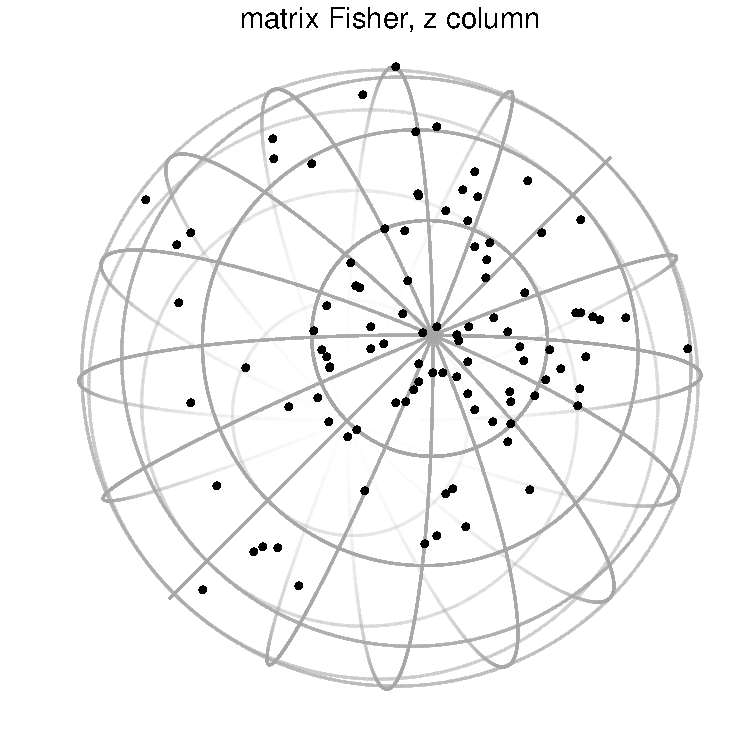
\includegraphics[width=.3\linewidth]{eye-fisher-3}
\caption{\label{fig:eye-fisher}Sphere plots for a sample of 100 rotations from a matrix Fisher distribution with circular variance $\nu=0.25$}
\end{figure}
\begin{figure}
\centering
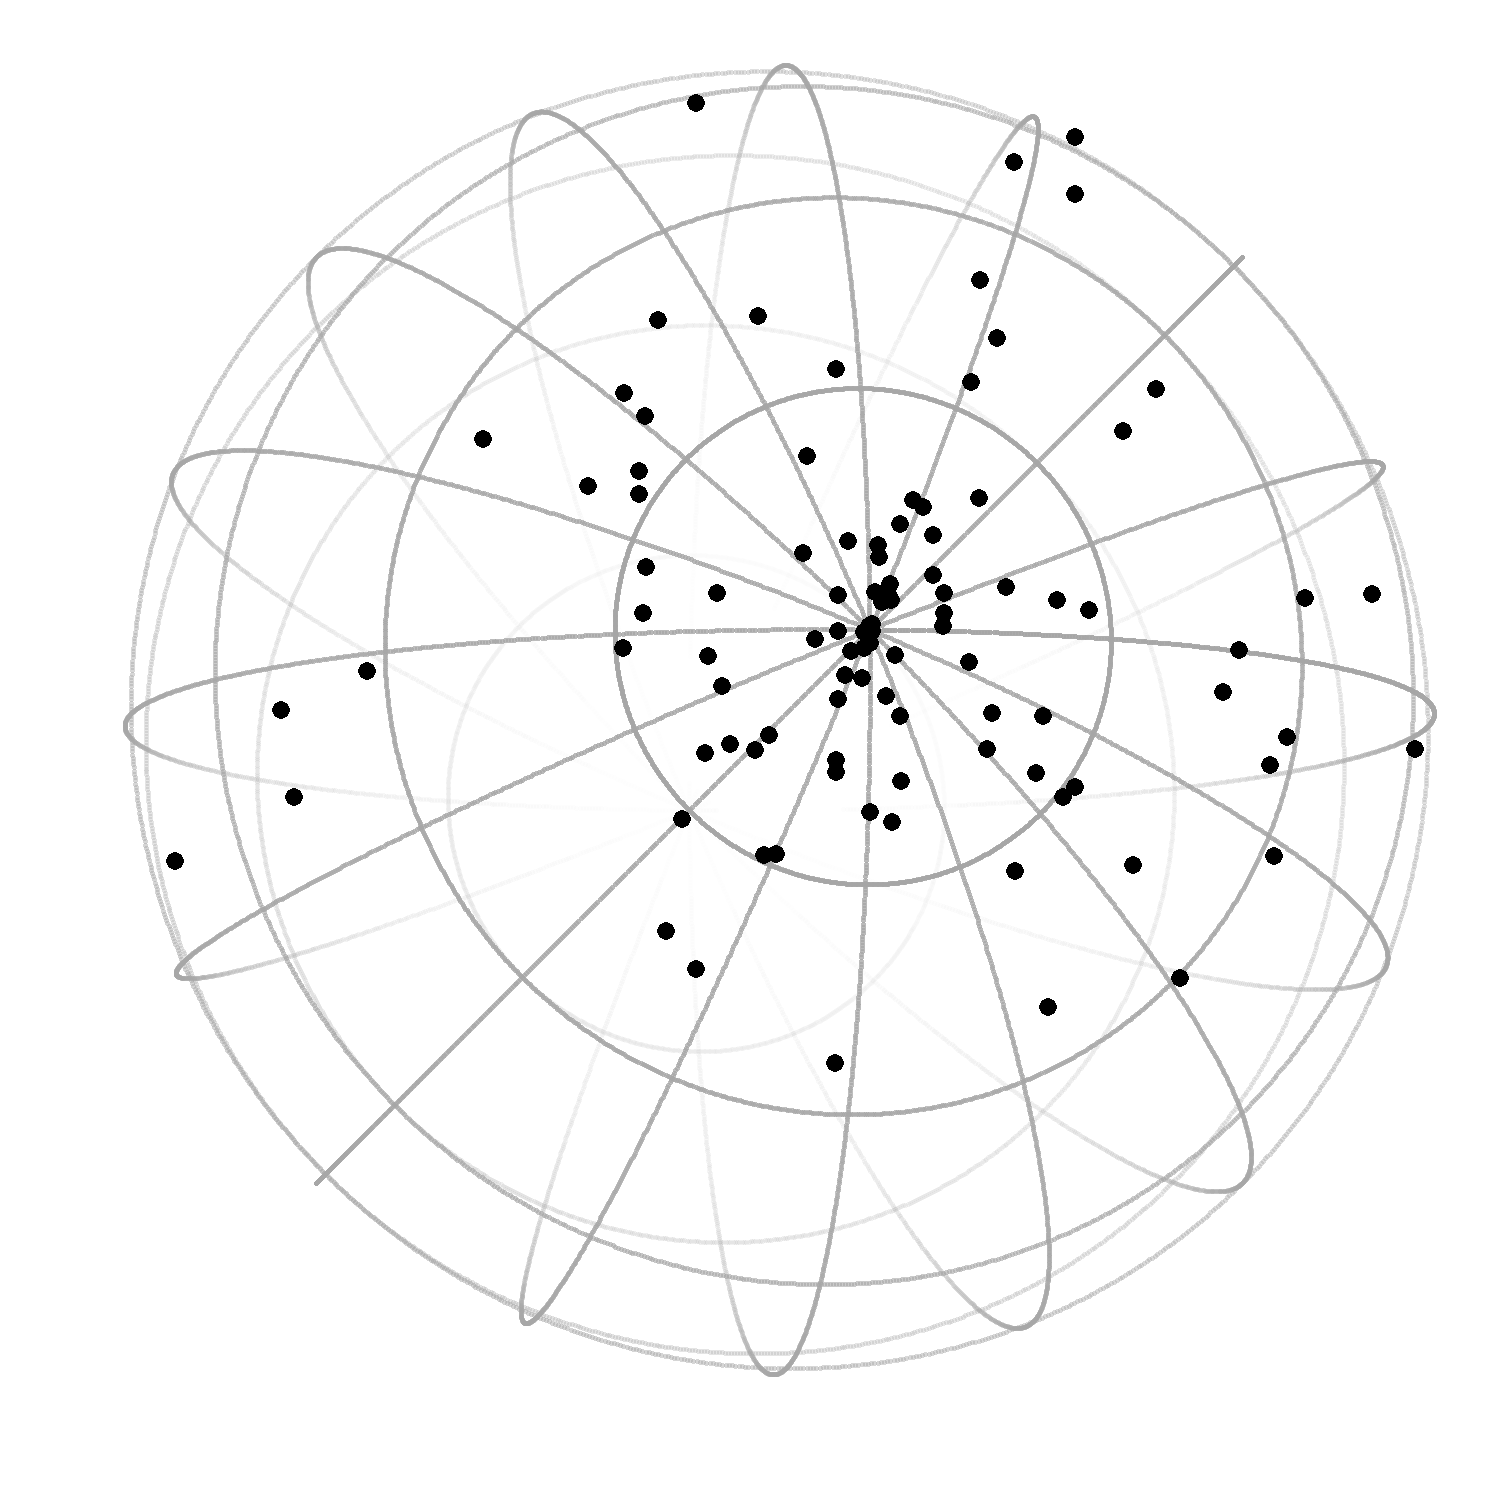
\includegraphics[width=.3\linewidth]{eye-vmises}
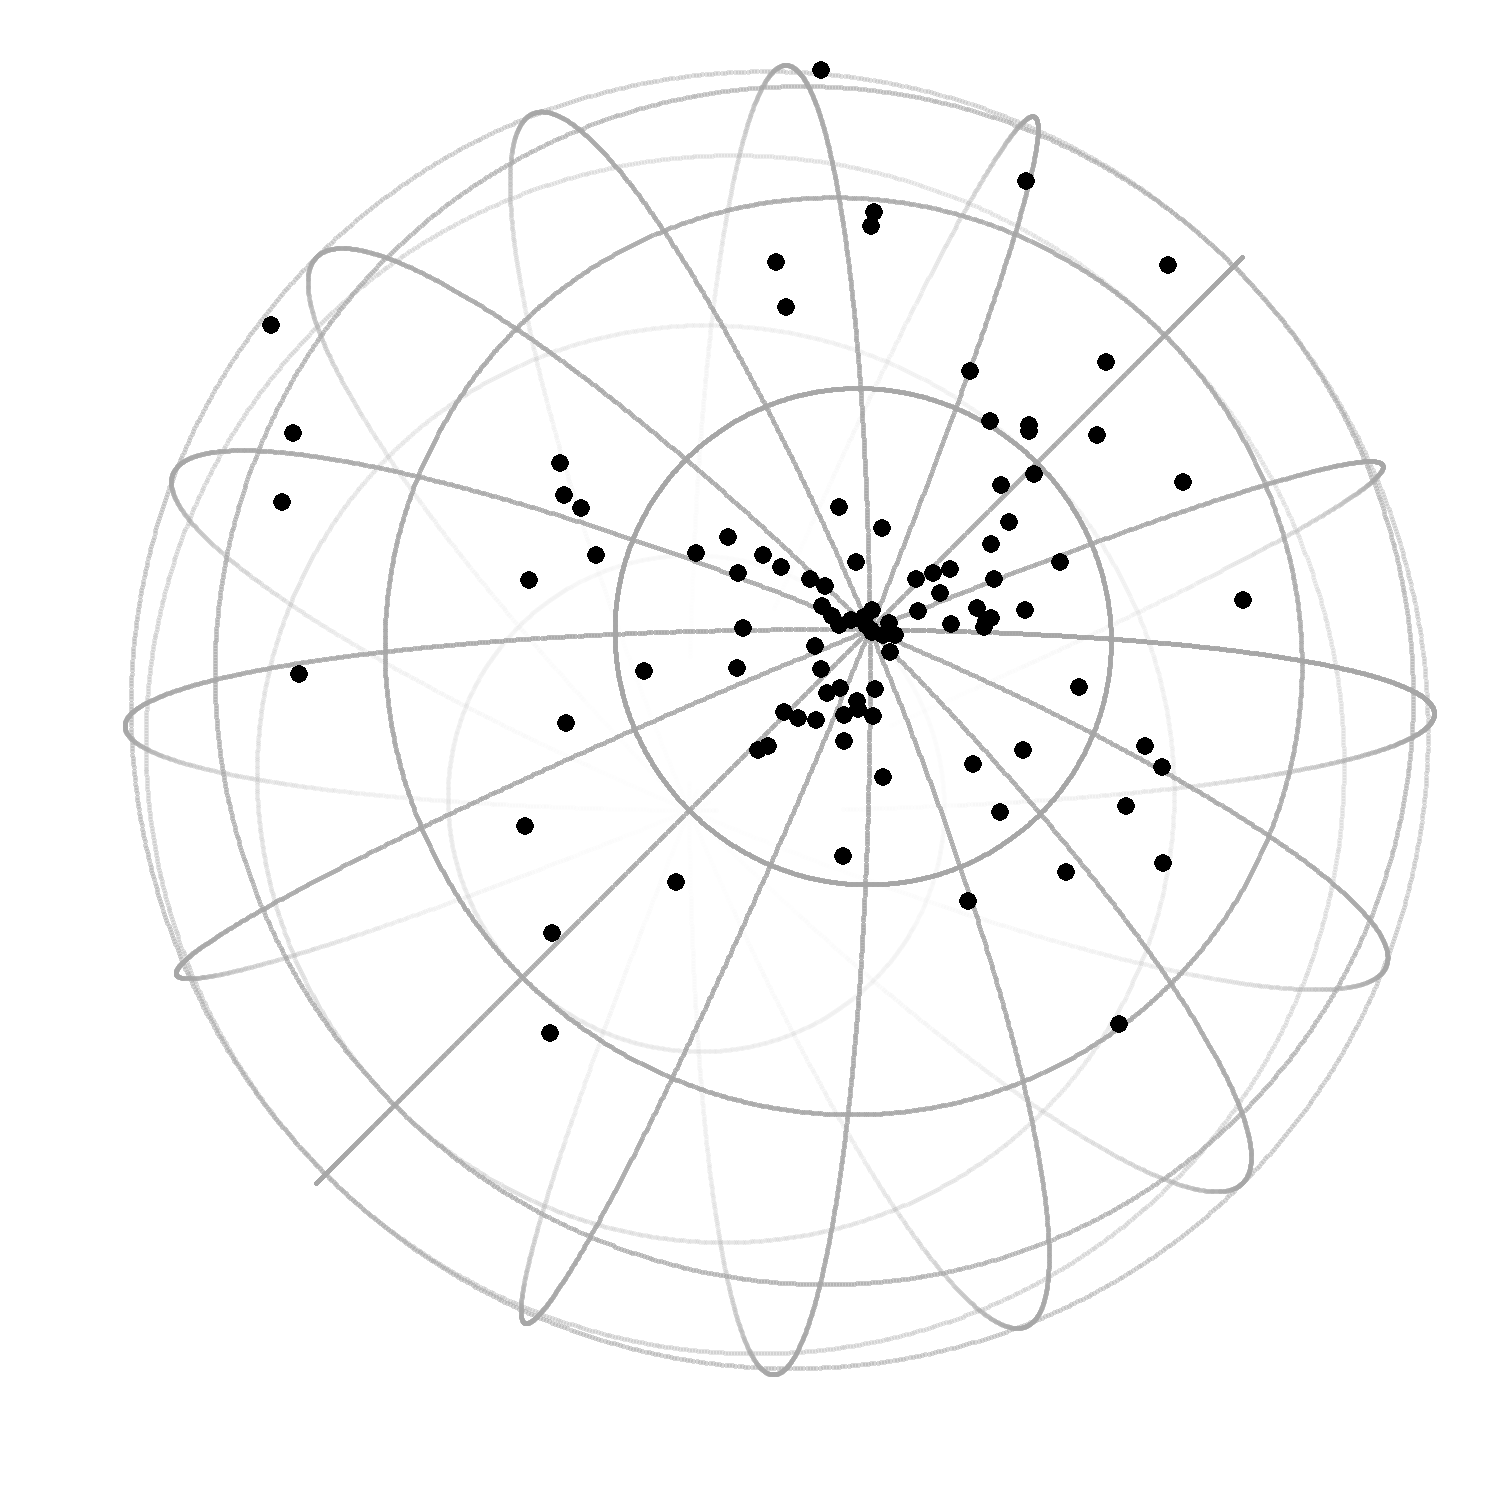
\includegraphics[width=.3\linewidth]{eye-vmises-2}
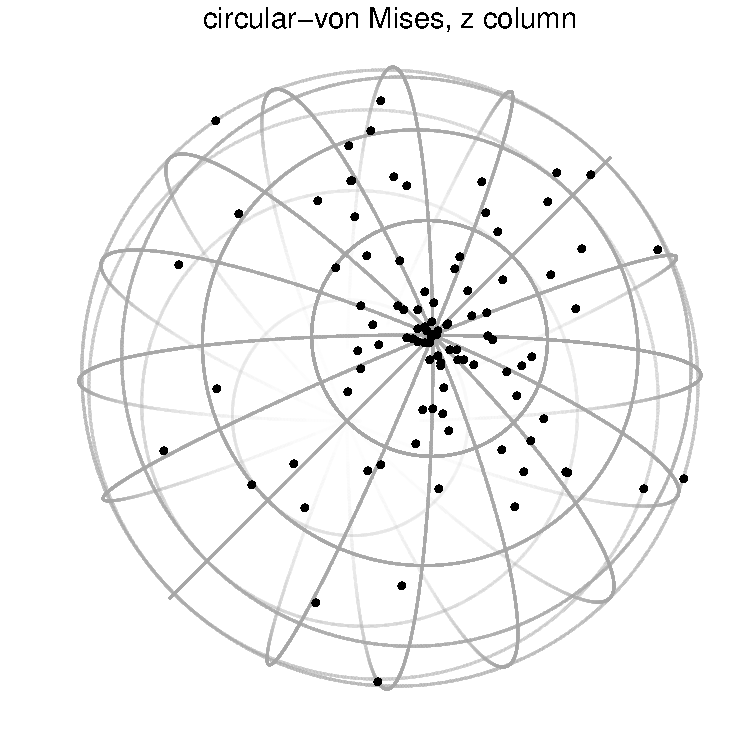
\includegraphics[width=.3\linewidth]{eye-vmises-3}
\caption{\label{fig:eye-vmises}Sphere plots for a sample of 100 rotations from a circular-von Mises distribution with circular variance $\nu=0.25$}
\end{figure}
\end{document}